\subsection{Theory and Procedure}

\FloatBarrier

\begin{figure}[h!]
	\centering
	\caption{Common-Drain Amplifier}
	\label{fig:cd_amp}
	\begin{circuitikz}
		\draw
		( 0 , 0 ) node[ nmos ] (my_nmos) {}
	
		% Gate
		(my_nmos.G) to [ short ] ++( -2 , 0 ) coordinate(g_out)
		(g_out) to [ V , v<=$V_{in}$ ] ++( 0 , -2 ) coordinate(gnd_1)
		(gnd_1) node[ ground ] (my_gnd_1) {}

		% Drain
		(my_nmos.D) to [ short ] ++( 2 , 0 ) coordinate(vcc)
		(vcc) to [ V , v<=$V_{DD}\rightarrow5V$ ] ++( 0 , -2 ) coordinate(gnd_3)
		(gnd_3) node[ ground ] (my_gnd_3) {}

		% Source
		(my_nmos.S) node [ ] (labeled_S) {$V_{out}$}
		(labeled_S) to [ R={$5k\Omega$} ] ++( 0 , -2 ) coordinate(my_e_gnd)
		(my_e_gnd) node[ ground ] (e_gnd) {}

		;
	\end{circuitikz}
\end{figure}

\FloatBarrier

A common-drain amplifier is to be constructed.
$V_{in}$ is swept from $0$\si{\volt} to $5$\si{\volt}.
The following is the saturation condition for the NMOS transistor:

\begin{equation}
	\label{eq:sat_cond_nmos}
	V_{DS} > V_{GS} - V_T \rightarrow V_{D} > V_{G} - V_T \rightarrow V_{in} < 5V + V_T
\end{equation}

So long as $V_{in}$ stays below $5$\si{\volt} and high enough that the MOSFET does not enter the cutoff region, it remains in saturation.
So, for small values of $V_{in}$, the transistor operates in the cutoff region because a current-enabling channel cannot form.
Once $V_{in}$ is high enough that the channel can form, the transistor operates in the saturation region due to the high drain voltage "pinching-off" the channel.
By design, $V_{in}$ never exceeds $5$\si{\volt}. So, the transistor transitions from cutoff to saturation during the DC sweep.

\subsection{Results}

\FloatBarrier

\begin{figure}[h!]
	\centering
	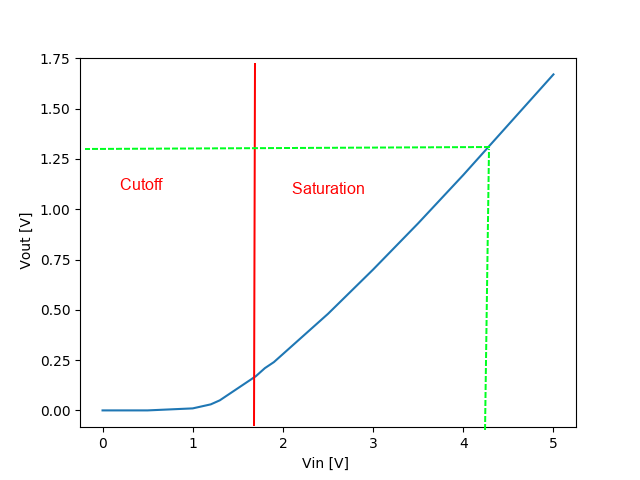
\includegraphics[scale=0.50]{../data/common_drain_edited.png}
	\caption{Common Drain Amplifier Voltage Transfer Characteristic}
	\label{fig:common_drain}
\end{figure}

\FloatBarrier

The amplifier should be biased in the middle of the saturation region. Using the characteristics of the NMOS determined earlier, the threshold voltage is taken to be $V_T = 1.7$\si{\volt}. Suppose the transistor exits the cutoff region for some $V_{in} > V_T$. Then, no current flows through the resistor. Therefore, the source voltage becomes $0$\si{\volt}, meaning that $V_{GS} = V_{in} > V_T$. This is a contradiction. Thus, transistor cannot begin to exit cutoff at a voltage above $V_T$. \\

For a voltage $V_{in} < V_T$, assume the transistor is not in cutoff. Then, current flows through the resistor.
Therefore, the source voltage is above ground, meaning that $V_{GS} = V_{in} - V_S < V_T$.
This is a contradiction.
So, the transistor exits cutoff mode when $V_{in} = V_T = 1.7$\si{\volt}. The current begins to rise from $0$\si{\milli\ampere} before this point.
However, $V_T = 1.7$\si{\volt} is used when calculating the edge between saturation and triode. For the sake of consistency, $V_T = 1.7$\si{\volt} is used for the edge between cutoff and saturation. \\

The transistor exits saturation when $V_{in} = 5V + V_T = 5V + 1.7V = 6.7V$. 
So, the midpoint of the saturation region occcurs when $V_{in} = \frac{1.7V + 6.7V}{2} = 4.2$\si{\volt}, which corresponds to a bias current of $\frac{V_{out}}{5k\Omega} \approx \frac{1.3V}{5k\Omega} = 0.26$\si{\milli\ampere}.
